\chapter{Theoretical framework}
Quantum computing is based on a general framework that does not depend on the physical platform. Here, important concept such as qubit, and quantum operations are described before showing how we can realize them, from a theoretical point of view, with trapped ions. The same goes with quantum networking, the concept and the realization can be treated separately and they will be described in this chapter. Furthermore, in this chapter we will take a look into Gaussian beams and their properties. Since that is the shape emitted by laser, it is important to understand their characteristic and how to manipulate them. Lastly Acousto-optical interactions are introduced and studied to give an idea of how AODs work and how they can be used to steer a laser beam.
\section{Quantum logic with trapped ions}
\subsection{Quantum computer and quantum gates}
The concepts of quantum computing are borrowed and extended from classical computational theory. In the classical case, information is represented in terms of binary digits, the so called bit, essentially mapping information to a base-2 number. Information processing is done with gates acting of those numbers. The idea of quantum computer is still to encode information in a binary form, but due to the nature of quantum mechanics, a quantum bit (in short qubit) gains new features that can be exploited to perform different kind of operations that in some cases are a speed up compared to the classical case.\\
A qubit is formally a normalized wave function that can be written as superposition of two orthogonal states indicated usually with $\ket{0}$ and $\ket{1}$:
\begin{equation}
\label{qubit}
\ket{\psi} = \alpha \ket{0} + \beta\ket{1},
\end{equation}
where $\alpha,\beta$ are probability amplitudes, two complex numbers that satisfy the relationship $|\alpha|^2+|\beta|^2 = 1$.
At first glance, the advantage of qubits seems obvious, while one classical bit can store only one bit of information, a qubit can be in any linear combination, i.e. $\alpha$ and $\beta$ can be chosen freely and any information can be represented. Although, the reality is different, due to rules of quantum mechanics, $\alpha$ and $\beta$ cannot be directly accessed, which means that we can get only a limited amount of information out of a qubit. The outcome of measuring a qubit will give the value 0 with a probability of $|\alpha|^2$ and 1 with a probability of $|\beta^2|$.  [..]

Qubits also have a geometrical representation that can be useful, equation \eqref{qubit} depends on 4 real numbers, however since $\psi$ is normalized, we can rewrite the expression as
\begin{equation}
\ket{\psi} = e^{i\gamma}\left(\cos\frac{\theta}{2}\ket{0} + e^{i\varphi}\sin\frac{\theta}{2}\ket{1}\right).
\end{equation}
the global phase factor $e^{i\gamma}$ can be left out, as it does not influence the measurement outcome. This leaves us with only two real number: $\theta$ and $\varphi$. A qubit is therefore representable with only these two numbers that we can chose to represent geometrically with normalized spherical coordinates. The so called Bloch sphere is depicted in figure \ref{blochsphere}, every point on its surface represents a different state of the qubit. Here qubit manipulation can be visualized as trajectories on the surface, which in some cases is very useful. The drawback of this representation is that it is limited to only one qubit, so it loses usefulness when dealing with multiple qubits.
\begin{figure}[H]
\centering
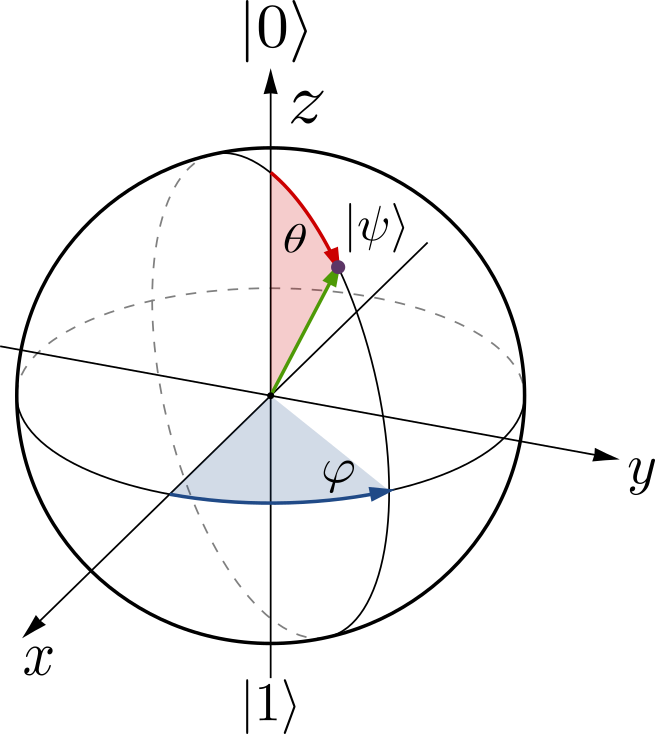
\includegraphics[width = .4\textwidth]{bloch_sphere}
\caption{The Bloch sphere. The states $\ket{0}$ and $\ket{1}$ are at the poles of the sphere, every other point of the surface represents a superpositions of these states. A quantum gate can be seen as trajectory on the surface mapping one state to another.}
\label{blochsphere}
\end{figure}

A more practical way of dealing with qubits is via matrices. We can assign to the states $\ket{0}$ and $\ket{1}$ the following:
\begin{equation}
\ket{0} = \begin{pmatrix}
 1 \\
 0
\end{pmatrix} \quad
\ket{1} = \begin{pmatrix}
 0 \\
 1
\end{pmatrix} \implies \ket{\psi} = \begin{pmatrix}
 \alpha \\
 \beta
\end{pmatrix}.
\end{equation}
In this representation, manipulations of qubits are easily calculated using $2\times2$ unitary matrices. These kind of operations are named \emph{quantum gates} and they are the building blocks of quantum computing. Every quantum algorithm can be written as a sequence of quantum gates and it is therefore important to understand them. For a single qubit any gate can be written as combination of two operations \cite{hempel}
\begin{equation}
U_z(\theta) =  \begin{pmatrix}
 e^{-i\frac{\theta}{2}} & 0 \\
 0 & e^{i\frac{\theta}{2}}
\end{pmatrix} \qquad U_\varphi(\theta) = \begin{pmatrix}
\cos\frac{\theta}{2} & -i e^{-i\varphi}\sin\frac{\theta}{2} \\
-ie^{i\theta}\sin\frac{\theta}{2} & \cos\frac{\theta}{2}
\end{pmatrix}.
\end{equation}
These two matrices can be seen as two different rotations in the Bloch sphere, $U_z$ is a rotation around the $z$ axis by the amount $\theta$, while $U_\varphi$ is a rotation on the $x-y$ plane around an axis tilted by $\varphi$. examples [H gate, phase gate]\\
\newline
As we have seen, a single qubit has already the advantage of superposition compared to classical case. When considering multiple qubits, we gain even more quantum mechanical features like entanglement. This phenomenon does not have a classical analogy and it is an extremely useful tools in quantum information.\\
In general a state with $N$ qubits is written as tensor product of the single qubit states $\psi_i$
\begin{equation}
\ket{\psi_N} = \ket{\psi_1}\otimes \ket{\psi_2}\otimes \cdots \ket{\psi_N} \equiv \ket{\psi_1\psi_2\dots \psi_N}.
\end{equation}
If we had to write out explicitly all the probability coefficients of $\psi_N$, we would need $2^N$ complex numbers. It is clear then why classical computer cannot keep up. $N$ bits can only give $N^2$ different combinations, while the Hilbert space of qubits is exponentially larger.\\
Now, let us consider only 2 qubits, a particular case would be
\begin{equation}
\ket{\psi} = \frac{1}{\sqrt{2}}\left(\ket{00} + \ket{11}\right).
\end{equation}
If a measurement is made on one of the two qubit and, for instance, the outcome is 0, the wave function collapses to the state $\ket{00}$, collapsing also the state of the other qubit, even if no operation has been directly performed on it. Next you measure the the second qubit and the outcome will be 0 with unitary probability. Viceversa, if the outcome if the first measurement was 1, the state collapses to $\ket{11}$ and the outcome of the second measurement is always 1. The two qubits are correlated, but this correlations is stronger than the classical one.\\
Gates that involve multiple qubits are written as $2^N\times 2^N$ unitary matrices, a famous example is the CNOT gate, [..]

It can be shown [] that the examples we saw here, H gate, phase gate, and CNOT gate form a universal set of quantum gates, i.e. a sequence of these gates approximate every other quantum gate.

\subsection{Ion qubits and laser-ion interactions}
Qubits can be encoded in any pair of orthogonal states. In the case of an ion it is possible to take two internal electronic states. The choices are multiple: an optical qubit is implemented in an optical transition, an hyperfine qubit is between two hyperfine states, and a Zeeman qubit can be realized with two magnetically separated levels. We will take the choice of an optical qubit, in this case lasers provide an easy way to manipulate the population of the two level and therefore to manipulate the state of the qubit, implementing quantum gates in an almost straightforward way. As long as the chosen levels are well separated, and the light is near resonant to the transition, it is possible to describe the system with the basic 2-level atom scheme interacting with classical light. \\
In this section, the theoretical model of a 2-level atom is presented together with a model of interactions between the laser and the ion. This represents a physical implementation of the concepts illustrated in the previous section.
\begin{figure}[H]
\centering
\includegraphics[width = .4\textwidth]{2levelatom}
\caption{2-level atom scheme, the ground and excited states are denoted as $\ket{g}$, and $\ket{e}$. $\omega_l$ is the laser frequency, which is detuned by $\Delta$ from the transition frequency $\omega_0$.}
\label{2levelatom}
\end{figure}

Consider the system in figure \ref{2levelatom}, the Hamiltonian of the atomic part can be written as:
\begin{equation}
H_a = \hbar\omega_0 \ket{e}\bra{e},
\end{equation}
where $\omega_0$ is the frequency difference between the ground and excited state, the energy of the ground state has also been set to 0. The Hamiltonian of the interaction between light and atom can be written as []
\begin{equation}
H_{int} = -d\cdot E
\end{equation}


- 2 level atom scheme\\
- Model of laser-ion interaction: rabi flops, AC stark shift
\section{Quantum networking with trapped ions}
\subsection{General introduction}
Quantum networks can serve different purposes, either transmission of quantum information at long distances, or interconnections of quantum processors for qubits scaling. The topology of these configurations changes, but the constituent elements are the same: a node, where quantum information is prepared, manipulated, and stored; and a link that connects node and where information is transmitted. Links are typically realized with optical fibers, photons can carry quantum information over long distance with very high speed. Instead, nodes are realized in a variety of ways: trapped ions [], neutral atoms [], atomic ensembles [].\\
A fundamental property of quantum network is the ability of transmitting faithfully a superposition state between nodes. This is not easily achievable,






- Nodes, interface, link, protocols\\
- logic, memory, interface, Bell pairs, purification, multi-mode
- Distributed entanglement
\subsection{Cavity QED}
- Simple model atom in cavity: g,gamma, k
\section{Basics of ion trapping}
\subsection{Linear Paul trap}
In order to trap a charged atom, a three dimensional trapping potential $\phi$ is needed. However it follows directly from Maxwell equation $\nabla^2 \phi = 0$ that the potential must be antitrapping at least in one direction. There are two workarounds for this problem: the first one introduces magnetic fields to trap particles in some directions, this takes the name of Penning trap. The second solution is the so called Paul trap, and it is what we are going to describe in this section. The idea is to introduce a time varying potential, such that the antitrapping direction is constantly switching between two  different dimension. If the switching is timed correctly, the particle will not have the time to escape but will always encounter a potential barrier.
The shape of the trap can be adapted to load more ions in different geometries. For instance, a linear Paul trap is elongated in one direction where the trapping confinement is weaker, such that loaded ions will align in a single long string. This kind of trap is depicted in figure \ref{trap}.
\begin{figure}[H]
\centering
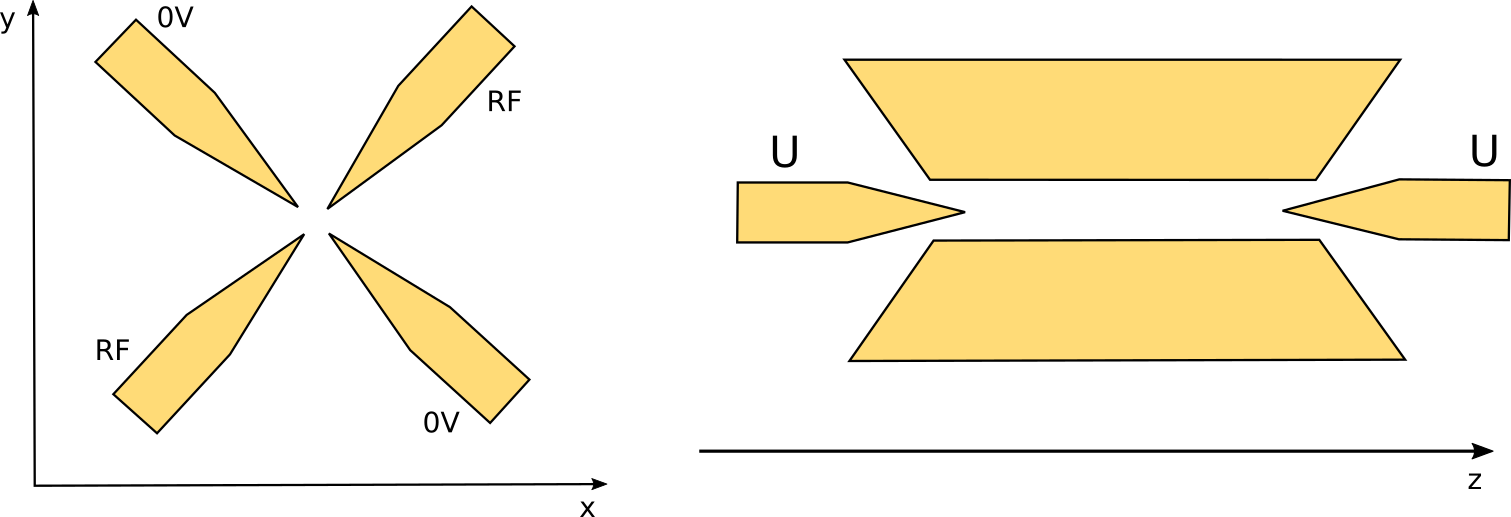
\includegraphics[width = .7\textwidth]{trap}
\caption{A linear paul trap. U is the voltage applied to the electrodes trapping in the $z$ direction, while in the $x-y$ plane trapping is achieved with a radio frequency signal. $r_0$ is the distance from the central axis to the RF electrodes.}
\label{trap}
\end{figure}
The confinement in the $x-y$ plane is provided by 4 electrodes, two of which are grounded and the other two are connected to a radio frequency source. This design is similar to a mass filter, with the difference of additional endcaps electrodes in the $z$ direction that plug the trap and confine also in axial direction.\\
The potential inside the trap can be described for the $x-y$ plan independently from the $z$ direction. In the case of a linear Paul trap the radial potential is \cite{traptheory}:
\begin{equation}
\phi  = \frac{\Phi_0}{2r_0^2}\left(x^2 - y^2\right),
\end{equation}
with the amplitude that consists of a static part $U$ and a dynamical one $\Phi_0 = U + V \cos(\Omega t)$.
The study of the particle's motion with mass $m$ and charge $e$ inside the trap can be done with classical physics, Newton's second law in this case is
\begin{equation}
m\ddot{x} = -q \frac{\partial \phi}{\partial x} = - \frac{ex}{r_0^2}\left(U + V \cos(\Omega t) \right),
\end{equation}
and similarly for $\ddot{y}$. This equation can be written in the form of Mathieu equation by defining two parameters:
\begin{equation}
a_x = \frac{4eU}{\Omega^2r_0^2m}, \quad q_x = \frac{2eV}{\Omega^2r_0^2m} \implies \ddot{x} +\frac{\Omega}{4} \left(a_x + 2q_x \cos(\Omega t )\right)x = 0
\end{equation}
and with a change of variable $\tau = \frac{\Omega t}{2}$ we end up with
\begin{equation}
\label{mathieu}
\frac{\partial^2 x}{\partial \tau^2}+\left(a_x + 2q_x \cos(2\tau)\right)x = 0
\end{equation}
This kind of equations have stable solutions that can be found in a recursive way with Floquet theorem \cite{iondynamic}. However, the problem is simplified by performing the so called secular approximation, which consists of separating the motion in a slow changing position: $\bar{x}$ called \emph{secular motion}, and in a rapid oscillation: $\xi$, called \emph{micromotion}. The behaviour of micromotion is dictated by the force due to the potential at the position $\bar{x}$, and the secular motion will follow a time average of the potential $\langle \phi(t) \rangle$ eliminating therefore the effect of micromotion. In this case, equation \eqref{mathieu} becomes
\begin{equation}
\frac{\partial^2 \bar{x}}{\partial \tau^2} + \left(a_x + 2q_x \langle\cos(2\tau)\rangle\right)\bar{x} = 0
\end{equation}

\begin{figure}[H]
\centering
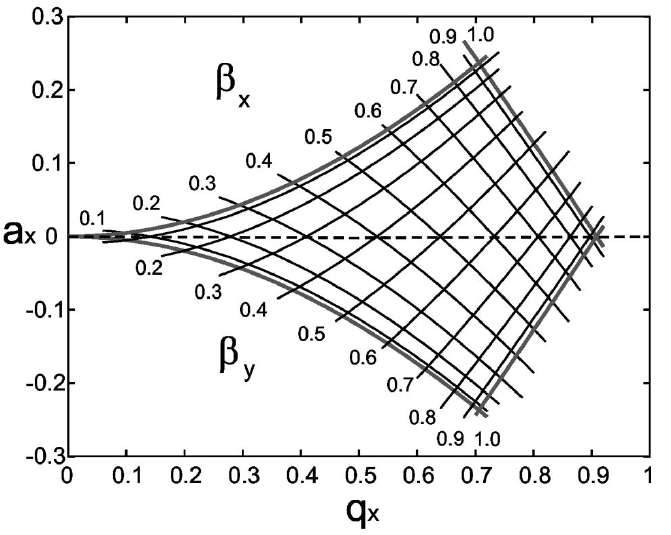
\includegraphics[width = .7\textwidth]{stabilitydiagram}
\caption{Stability diagram for a linear Paul trap, taken from \cite{iondynamic}. The coefficient $\beta_x,\beta_y$ can be calculated numerically from $a_x$ and $q_x$}
\label{stabilitydiagram}
\end{figure}


\subsection{Ion strings}
We have seen that the potential inside the trap can be described as an harmonic potential. What we are interested in, is the ion separation between $N$ ions loaded in the trap. This will give us an idea of how narrowly the beam should be focused and will set an appropriate problem spatial scale.\\
Let us consider the $z$ direction where the ions are weakly confined and will form a string. The potential can be approximated as harmonic and hence given by
\begin{equation}
V = \sum_{i=0}^N \frac{1}{2}M\omega^2z_i^2 + \sum_{i\neq j}^N\frac{Z^2e^2}{8\pi \epsilon_0}\frac{1}{|z_i-z_j|}
\end{equation}
The equilibrium position can be found at the minima of the potential, i.e. where the first derivative zeros
\begin{equation}
\frac{\partial V}{\partial z_i} = 0 \implies u_i - \sum_{j=1}^{i-1} \frac{1}{(u_i-u_j)^2} + \sum_{j= i+1}^{N} \frac{1}{(u_i-u_j)^2}= 0,
\end{equation}
where we defined the dimensionless quantity $u_i = z_i/l$ and $l^3 = \displaystyle\frac{Z^2 e^2 }{4\pi \epsilon_0 M\omega^2}$.
The last equations can be solved analytically only for 2 or 3 ions. In fact, for the case $N=2$ we simply get the system
\begin{equation}
\begin{cases}
  u_1 + \frac{1}{(u_1-u_2)^2} = 0\\
  u_2 - \frac{1}{(u_1-u_2)^2} = 0
  \end{cases} \quad \implies \quad u_1 = -u_2,\quad  u_1 = \left(\frac{1}{2}\right)^{2/3} \simeq 0.629
\end{equation}
For calcium-40 ions in a Paul trap with axial confinement of $\omega = 1$ MHz, we have $l \simeq 4.45\times 10^{-6}\,$m, which means that 2 ions are separated by $\simeq 5.6\, \mu$m. In the case of more ions the separation is lesser with the same confinement, but it is also possible to lower the axial frequency and increase the separation between the ions such that also in the case of several ions, the distance between them is still in the order of several $\mu$m. This size is accessible with current focusing optics and it is above the diffraction limit.\\
For more ions, a numerical approach has to be used, \cite{ion_spacing} reports values of $u_i$ up to $N=10$, and gives an empirical formula of the minimum separation
\begin{equation}
u_{min}(N) \simeq \frac{2.018}{N^{0.559}},
\end{equation}
Although, numerical solution are preferred and can be computed fast.
\subsection{Doppler cooling and detection}
\section{Laser beam}
\subsection{Gaussian beams}
Lasers emit light in the shape of Gaussian beams, so it is import to understand what Gaussian beams are and their characteristics. In this chapter we will take a closer look into such beams and introduce important quantities to characterize a Gaussian beam. \\
From a theoretical point of view, Gaussian beams are solution of the Helmholtz equation $(\nabla^2 + k^2)U(r) = 0$, with $k$ being the wavevector. Such equation is a time independent variant of the wave equation that follows directly from Maxwell equations. A paraxial approximation is often used, i.e.  we assume that the amplitude $A(r)$ of the wave is slowly varying, this means that the envelope of the wave is approximately constant on a length of $\lambda$ and we can write the complex electric field as $U(r) = A(r)e^{-ikz}$. If we can consider a wave propagating in the $z$ direction, we can find a solution in the form of \cite{saleh}:
\begin{equation}
\label{gaussianbeams}
U(r) = A_0 \frac{W_0}{W(z)}\exp\left\{-\frac{x^2+y^2}{W^2(z)}\right\}\exp\left\{-ikz-ik\frac{x^2+y^2}{2R(z)}+i\arctan(z/z_0)\right\}.
\end{equation}
 These solutions are called Gaussian beams, they are characterized by an amplitude $A$, a width $W(z)$, Rayleigh range $z_0$, and a curvature radius $R(z)$. Let us take a look at the features that arise from these beams. The optical power can be calculate by taking the square of the complex amplitude
\begin{equation}
\label{beamintensity}
I(r) = |U(r)|^2 = I_0 \left(\frac{W_0}{W(z)}\right)^2 \exp\left\{\frac{2x^2 + 2y^2}{W^2(z)}\right\}  \qquad I_0 = |A_0|^2.
\end{equation}
It is clear from here why the beam is called Gaussian. For a fixed $z$, the beam shape is the one of a two dimensional beam profile, i.e. the sections in the $x-y$ plane of a Gaussian beams are Gaussian shaped distribution. If we further take a cross section in the $x-y$ plane, we end up with a one dimensional Gaussian distribution. This shape is shown in figure \ref{gauss}, along with some important parameters.
\begin{figure}[H]
\centering
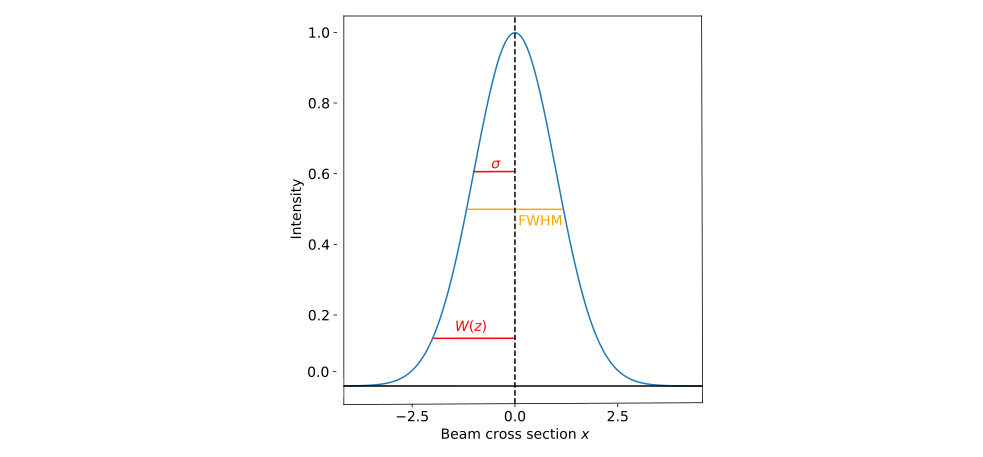
\includegraphics[width = .6\textwidth]{gauss}
\caption{Normalized Gaussian profile. Different ways of measuring the width of the profile are displayed geometrically.}
\label{gauss}
\end{figure}
It is important to understand how to characterize the width of a Gaussian shape, as it provides a quantitative way of measuring a laser beam width and its focus spot. A common way to define the width of a Gaussian distribution is according to the standard deviation $\sigma$, in this case the shape is given by $Ae^{-\frac{x^2}{2\sigma^2}}$, but for the intensity of a Gaussian beam, $W(z)$ is a much more used value. $W(z)$ is defined as the point at which the irradiance $I$ has fallen to $1/e^2 = 13.5\%$ of its maximum value. The relationship between these two quantities is easily found: $W(z) = 2\sigma$.\\
Another common parameter to characterize the width of a Gaussian is the full width half maximum (FWHM), this can be found to be related to $W$ as: $W = 0.84\cdot \text{FWHM}$. All these methods are equivalent and are different only from a prefactor, so for the rest of the section, we can stick to $W(z)$ and study its behaviour. Always from Helmholtz equation \cite{saleh}, the profile of $W(z)$ is found to be
\begin{equation}
W(z) = W_0 \sqrt{1 + \left(\frac{z}{z_0}\right)^2}\qquad W_0 = \sqrt{\frac{\lambda z_0}{\pi}}.
\end{equation}
This equation is plotted in figure \eqref{gaussprofile}.
\begin{figure}[H]
\centering
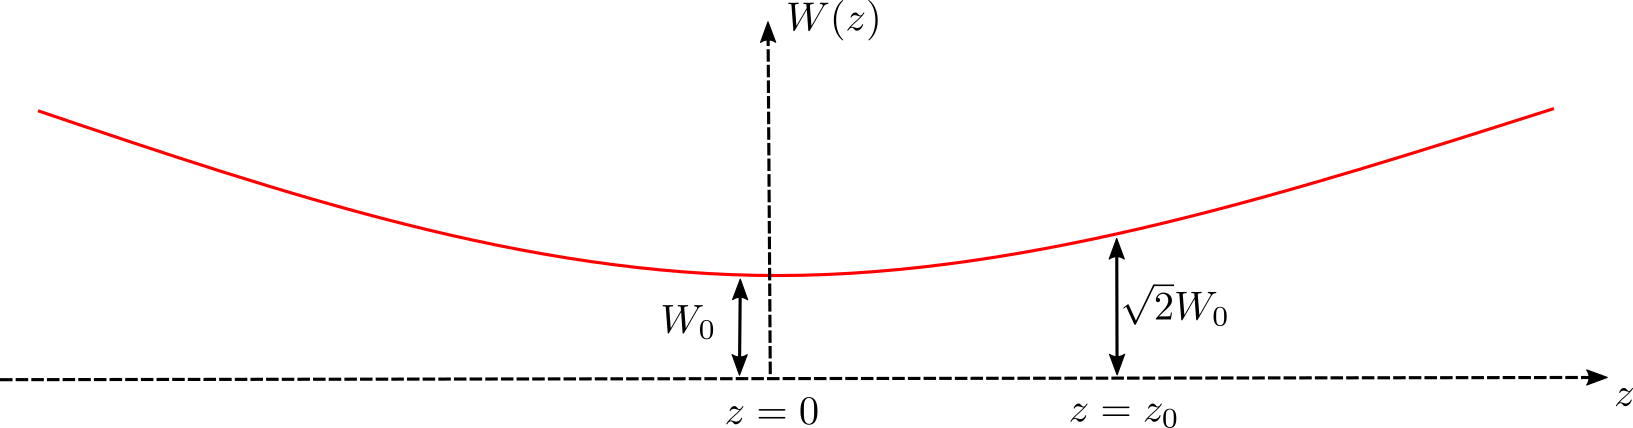
\includegraphics[width = \textwidth]{gaussprofile}
\caption{Width profile of a Gaussian beam. The beam is focused at the position $z_0$, here it assumes the minimum width $W_0$, also referred to as waist.}
\label{gaussprofile}
\end{figure}
There are several important features that can be seen. First of all, the width reaches a minimum in $z=0$ at a value of $W_0$, this is called focus of the beam and its width is the waist of the beam. Before and after the focus, the beam profile diverges almost linearly with an angle given by $\theta = W_0/z_0$, which means the smaller the focus, the greater it diverges. This property will become important later in the work, because it provides one limit on the focus spot. In fact, the optical aperture of the trap is limited by the electrodes, and a too diverging beam can potentially clip on one electrode causing aberrations and scattered light in the whole trap.  The Rayleigh range $z_0$ also has a geometrical interpretation, it represents the point where the beam width is exactly $\sqrt{2}W_0$, along with $\theta$ this is a useful way to characterize how fast a beam diverges.\\

In real experiments, all of these beam quantities can be manipulated with a lens. A Gaussian beam can therefore be shaped at will using optical elements. In order to study such reshaping, let us consider a thin spherical lens with focal length $f$, and radius of curvature $R_l$ placed at position $z$. The effect of the lens on the beam is to give an extra phase factor to equation \eqref{gaussianbeams} equals to $k(x^2 + y^2)/2f$ \cite{beamparameters}. We can match the phase of the incoming and emerging waves
\begin{equation}
kz +k \frac{x^2+y^2}{2R} - \zeta  - k\frac{x^2 + y^2}{2f} = kz + k \frac{x^2+y^2}{2R'} - \zeta \implies \frac{1}{R'} = \frac{1}{R} - \frac{1}{f}.
\end{equation}
The effect of the lens is now clear, it changes the radius of curvature to $R'$ according to the previous equation. Moreover, the width of the beam at the lens is not altered $W=W'$. Using these last two facts, we can determine all the parameters of the outgoing wave. The most important for us is the new waist $W_0'$
\begin{equation}
W_0' = MW_0 \qquad M = \frac{M_r}{\sqrt{q+r^2}} \qquad M_r = \left|\frac{f}{z-f}\right| \qquad r = \frac{z_0}{z-f}.
\end{equation}
$M$ is the magnification factor which provides an easy way to describe the change of the beam. For a better understanding of this last result, let us consider an less general example. We can place the lens at the focus $z=0$, and have a collimated beam $z_0 \to +\infty $. In this case the new waist is
\begin{equation}
W_0' = \frac{W_0}{\sqrt{1 + (z_0/f)^2}} \simeq W_0\frac{f}{z_0} = \frac{\lambda f}{\pi W_0}
\end{equation}
where the approximation comes from taking $z_0\gg f$. There are three parameters we can act on to achieve the smallest focus spot. The wavelength $\lambda$, the shorter the better. The focal length of the lens $f$ must be as small as possible, and the waist of the incoming beam $W_0$ as big as possible. Usually the wavelength is fixed in an optical system, so the best way to achieve a small focus is to collimate the beam as large as possible, the limit is given by the diameter $D$ of the lens. Hence, in the best case we have $D = 2W_0$ which means the waist is
\begin{equation}
W_0 = \frac{2\lambda}{\pi} \frac{f}{D}.
\end{equation}
A system focused to this limit is said to be diffraction limited. Indeed, if the size of the collimated beam is yet increased, the lens becomes a finite size aperture and diffraction effects will appear at the image plane. The next section will delve a little bit deeper in this kind of effects since it is the main limitation for the best achievable spot size.

\subsection{Diffraction limit}
There are some fundamental limits on how narrow a Gaussian beam can be focused, in this section we will take a look at what is the best achievable focus spot in the theoretical case with the best optics possible.
- To search whats limiting the diffraction, (lambda/2)
\subsection{Beam stearing via AOD's}
- How AODs work, simple Model\\
- Introduce diffraction efficiency, bandwidth
